\subsection{Lagrangian Perturbation Theory Validation (ex 3)}

\subsubsection{First-Order LPT}

The first step in validating the numerical implementation of First-Order Lagrangian Perturbation Theory (1LPT) is to examine the structure formation predicted by the Zel'dovich approximation (ZA). This provides a qualitative check of the particle displacement field and its ability to reproduce the large-scale structures generated by gravitational evolution.

\begin{figure}[htbp]
    \centering
    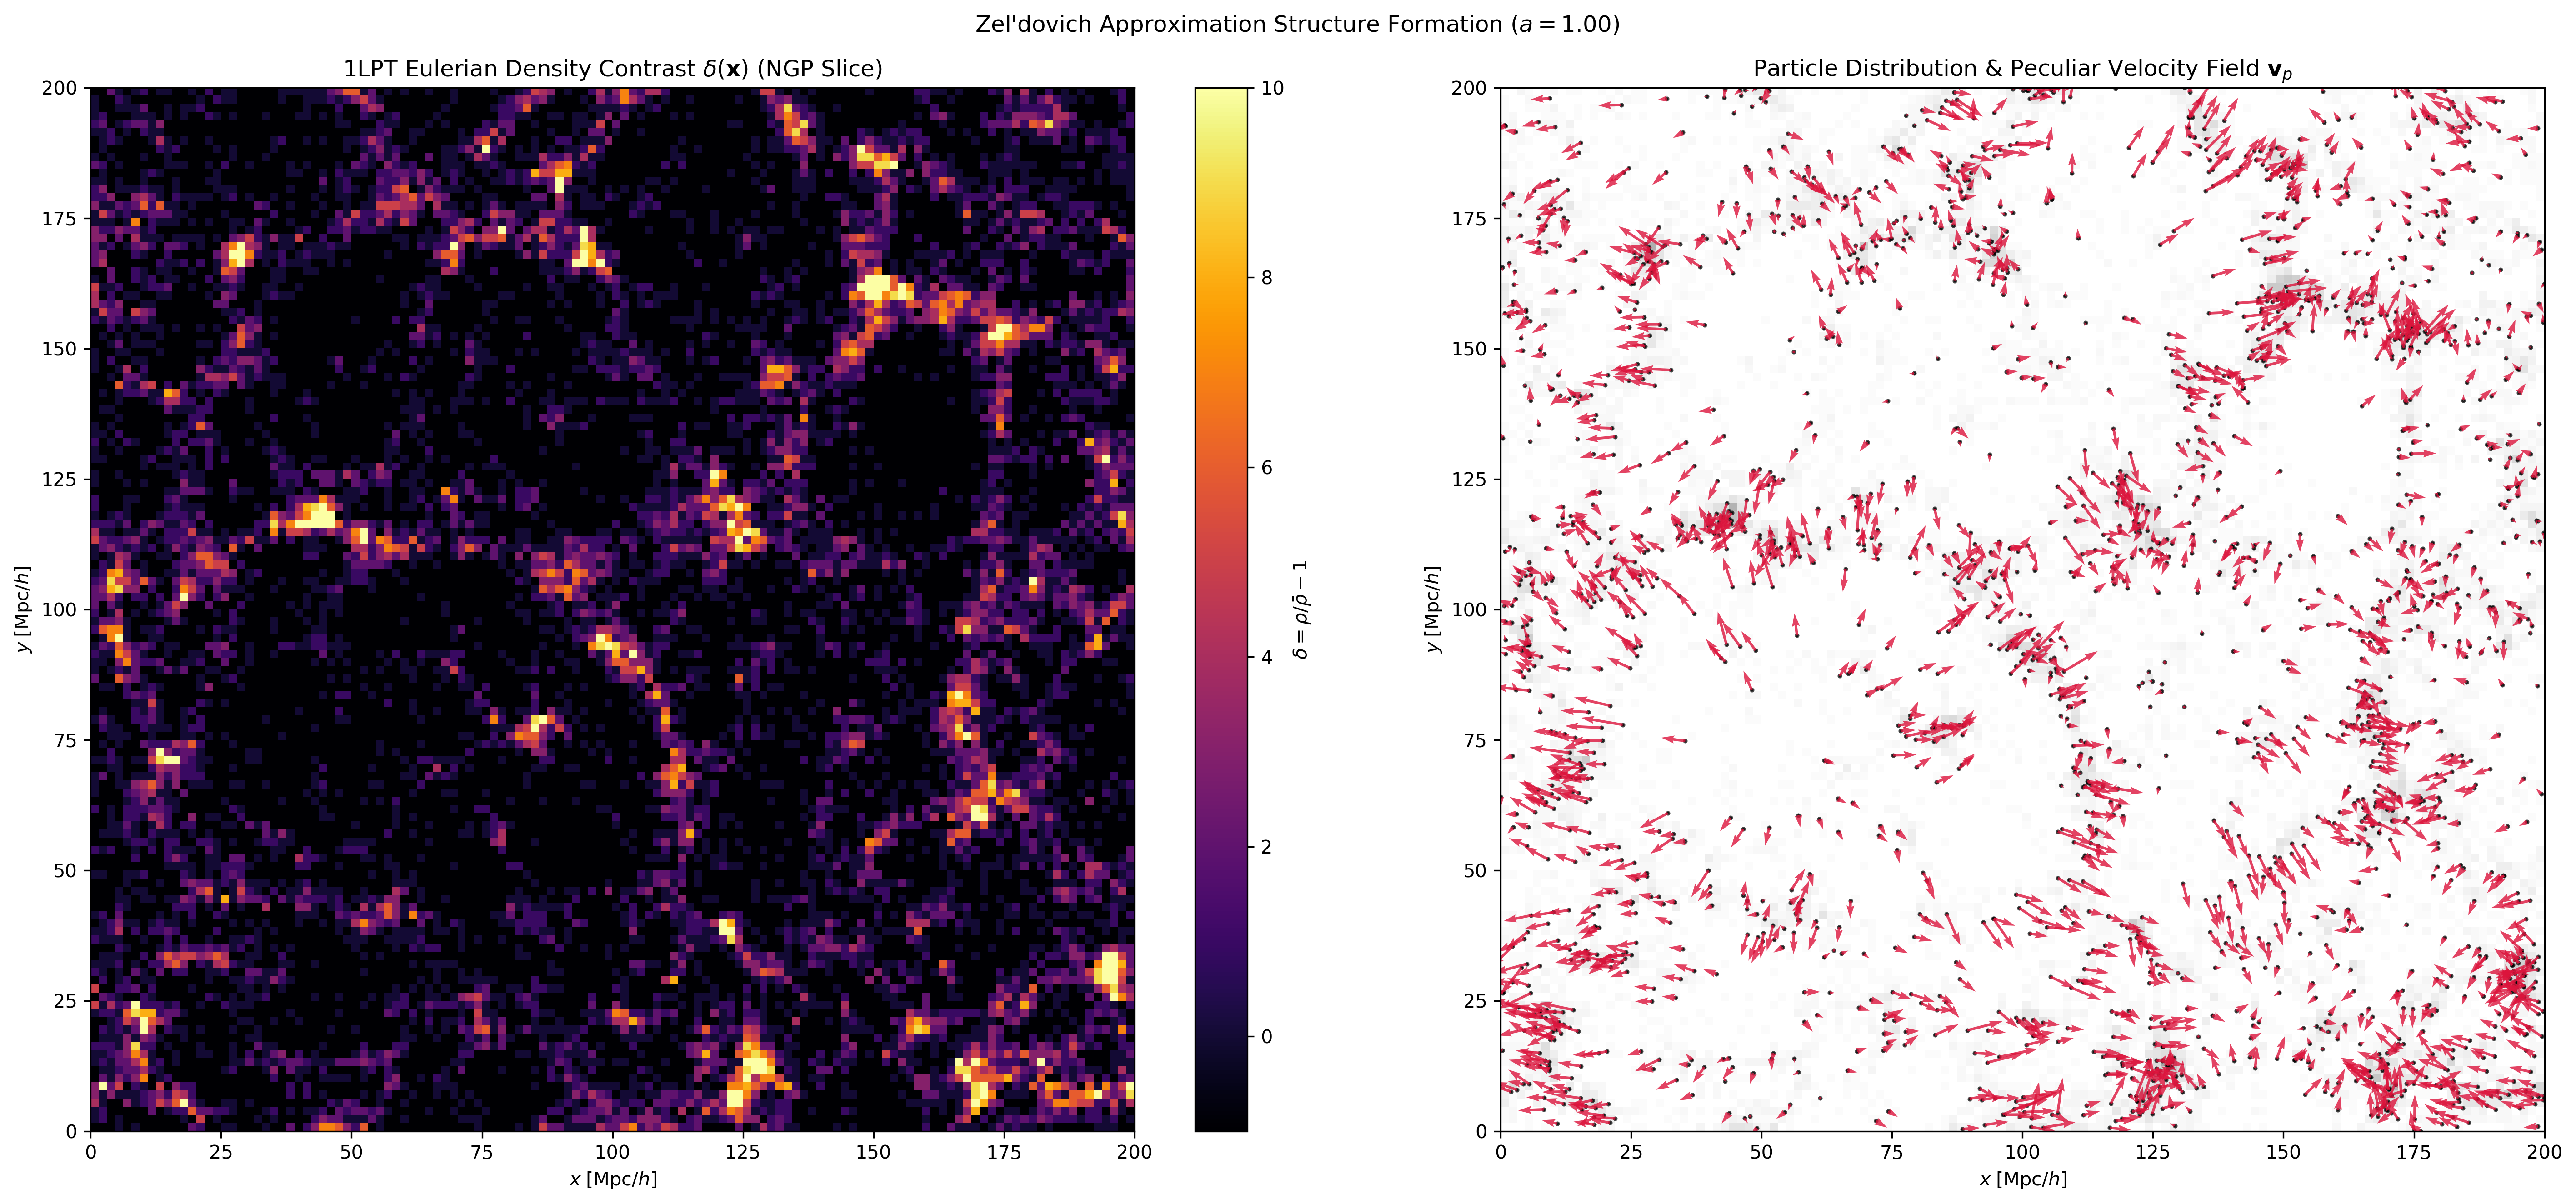
\includegraphics[width=0.82\textwidth]{New_Figures/Test_20261106_190746_lpt_cosmic_web_slice.png}
    \caption{Cosmic web structure produced by the numerical implementation of the Zel'dovich approximation.}
    \label{fig:ZA_implementation}
\end{figure}

Figure (\ref{fig:ZA_implementation}) shows the formation of filamentary and clustered structures characteristic of the cosmic web. This qualitative agreement provides an initial indication that the displacement field behaves as expected. Therefore, we also compare the measured matter power spectrum with the linear power spectrum generated by CAMB, using the reference linear spectrum \(P_{\mathrm{L}}(k,a_{\mathrm{ref}})\) and linear growth factor \(D_1(a_{\mathrm{ref}})\).

The first comparison examines the measured power spectra with the linear power spectrum:

\begin{figure}[H]
    \centering
    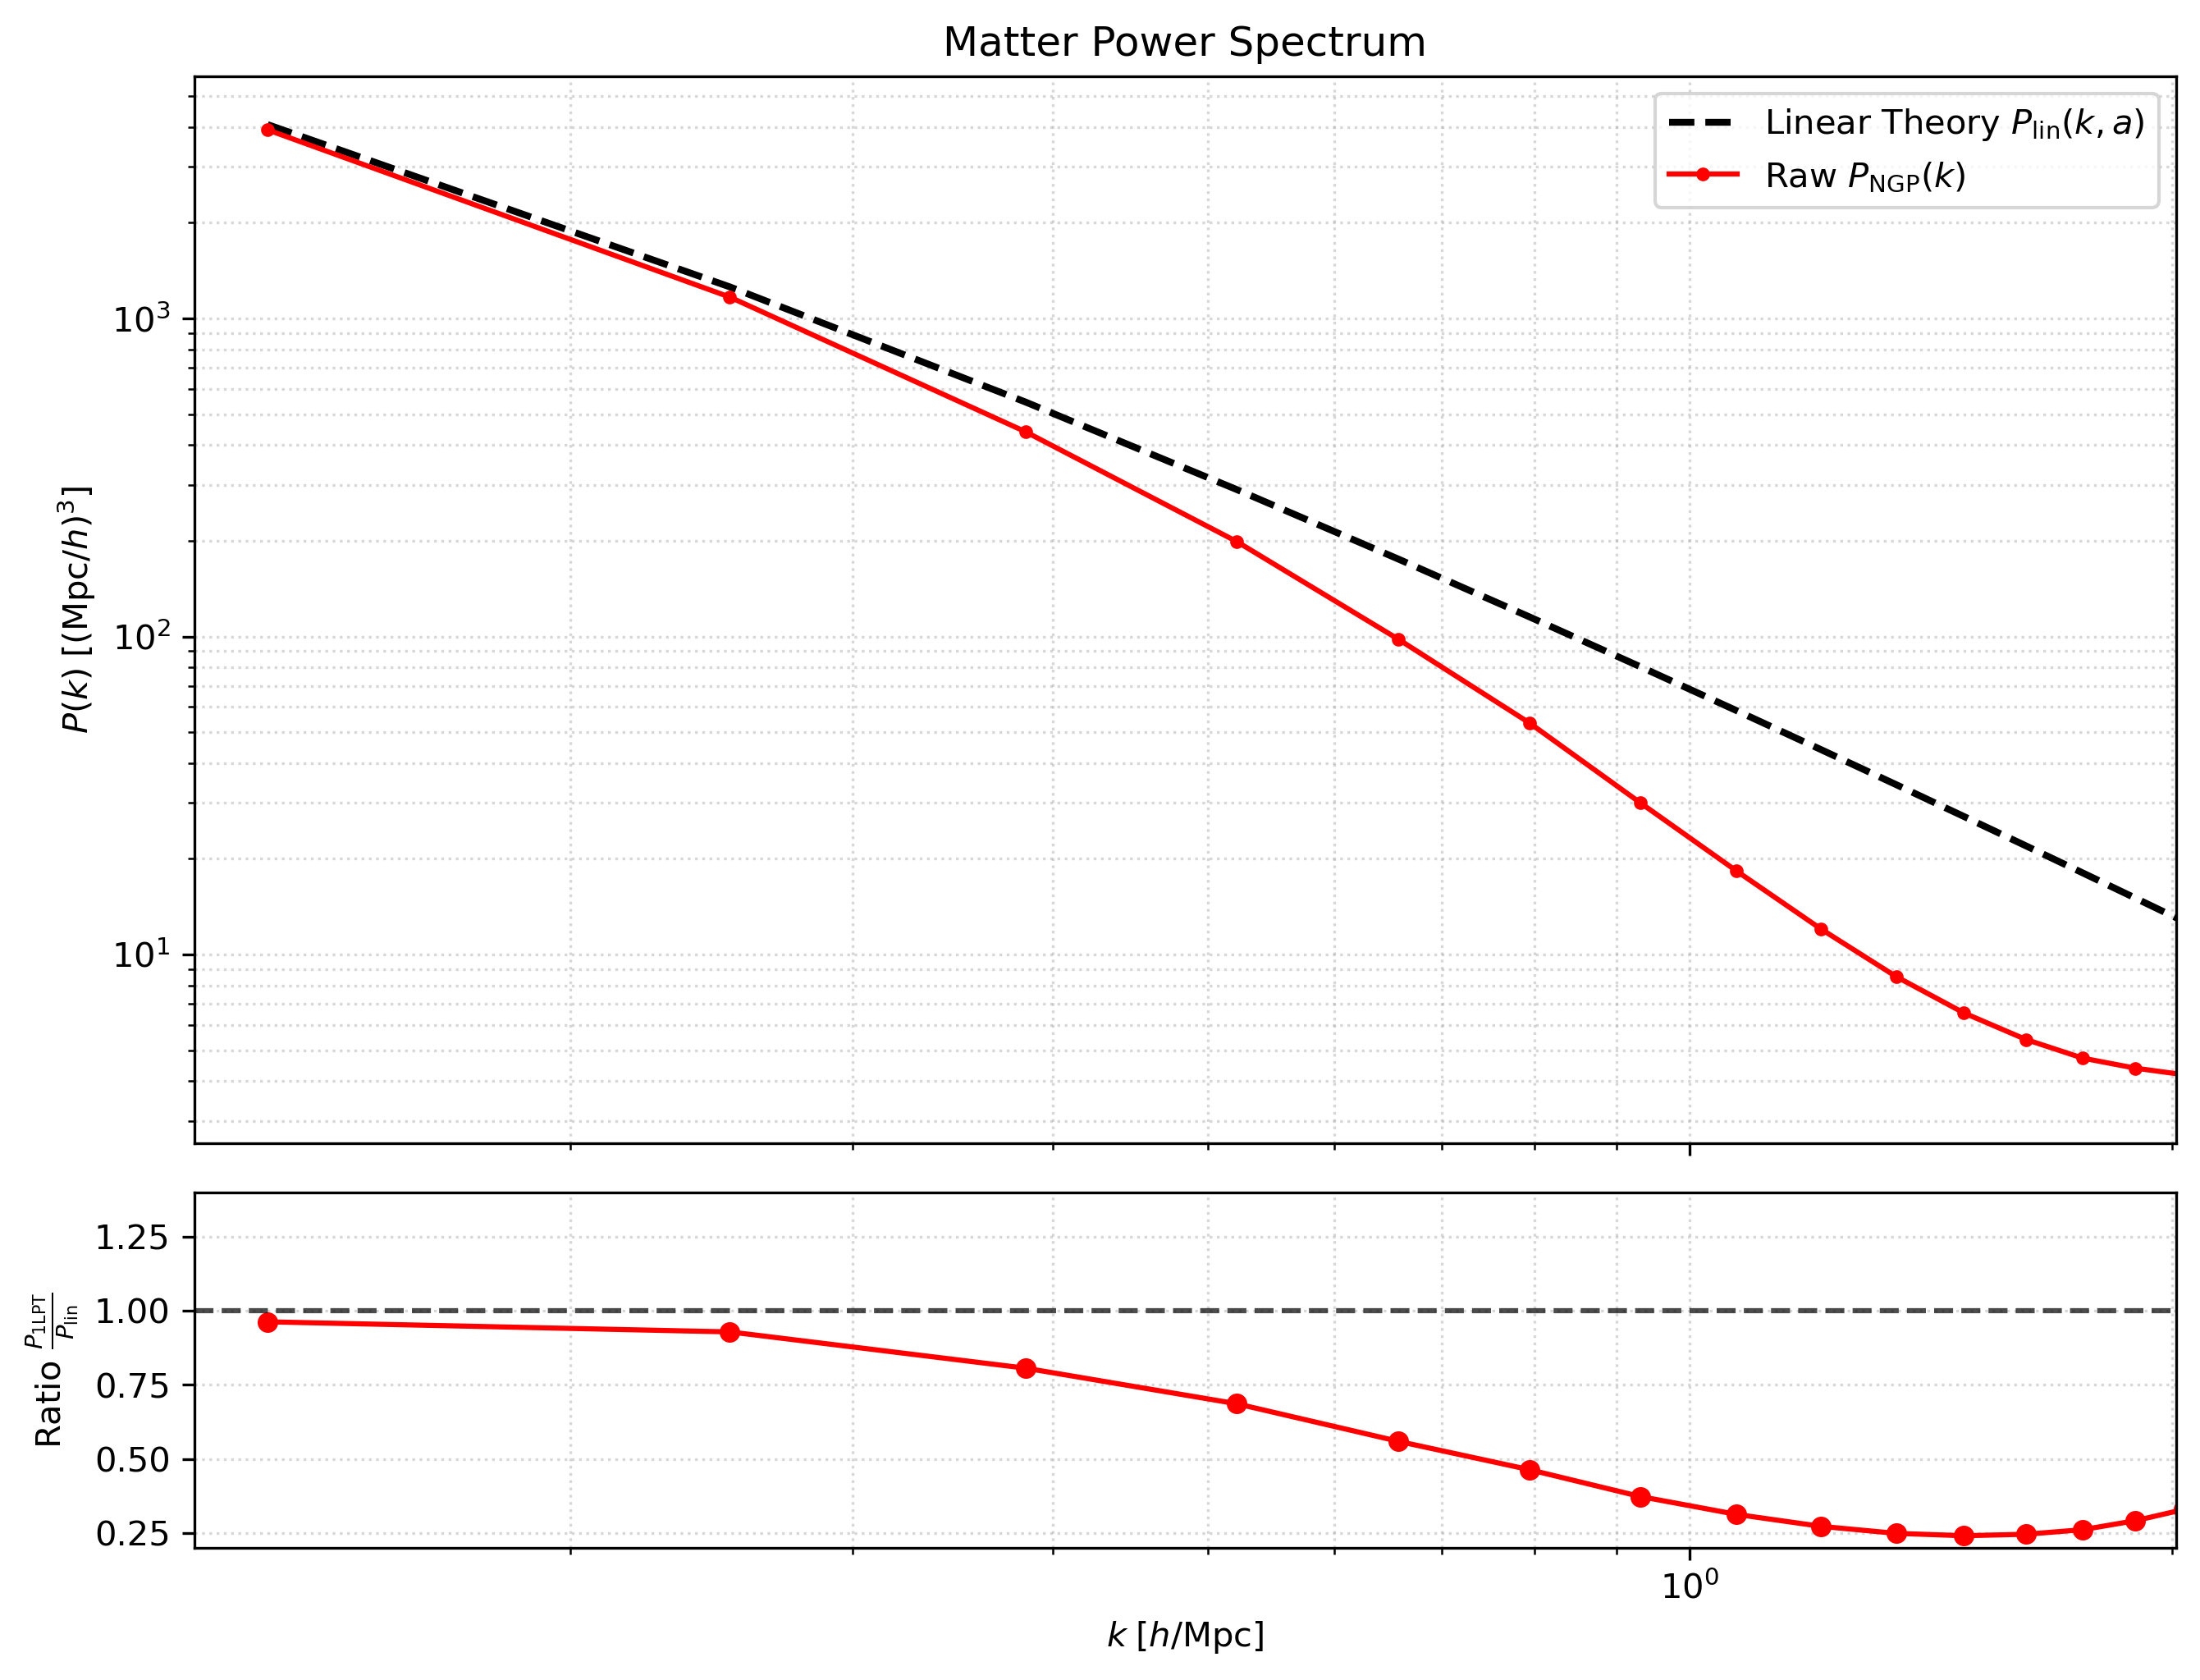
\includegraphics[width=0.82\textwidth]{New_Figures/Test_20261106_190746_lpt_power_spectrum.png}
    \caption{Comparison between the linear matter power spectrum and the power spectra measured}
    \label{fig:Power_spectrum_diff_}
\end{figure}

For a more detail analysis, we habe to compare different realizations. This allows us to investigate the dependence of the measured spectrum on the initial random realization and numerical resolution. Differences between the measured and theoretical spectra can arise from finite-volume effects, sampling variance, mass assignment onto the grid, and limitations associated with estimating power at large wavenumbers.

To obtain a more robust comparison, we average the measured spectra over ten random seeds for each grid resolution, considering \(N_g=64\), \(128\), and \(256\). We also account for the mass-assignment window function associated with depositing particles onto the grid. The squared Fourier-space window function is defined as

\begin{equation}
    |W(\mathbf{k})|^2 =
    \prod_{i=x,y,z}
    \left[
        \operatorname{sinc}\left(
            \frac{k_i \Delta x}{2\pi}
        \right)
    \right]^{2p},
    \label{eq:mass_assignment_window}
\end{equation}

where \(\Delta x=L/N_g\) is the grid spacing, \(p\) is the order of the mass-assignment scheme, and \(\operatorname{sinc}(x)=\sin(\pi x)/(\pi x)\) is the normalized sinc function. This expression describes the suppression of Fourier modes introduced by mass assignment. Since the power spectrum is proportional to the squared modulus of the Fourier-space density contrast, \(P(k)\propto|\delta(\mathbf{k})|^2\), the corresponding power-spectrum window is \(|W(\mathbf{k})|^2\).

When appropriate, the measured spectrum can be corrected for this effect by dividing by the squared window function. Such a correction is particularly relevant at high wavenumbers, where mass assignment can significantly suppress the measured power. However, this correction does not eliminate other sources of numerical error, such as aliasing. The resulting comparison, combining multiple realizations and grid resolutions, is shown in Figure(\ref{fig:Power_spectrum_diff_Ng}):

\begin{figure}[H]
    \centering
    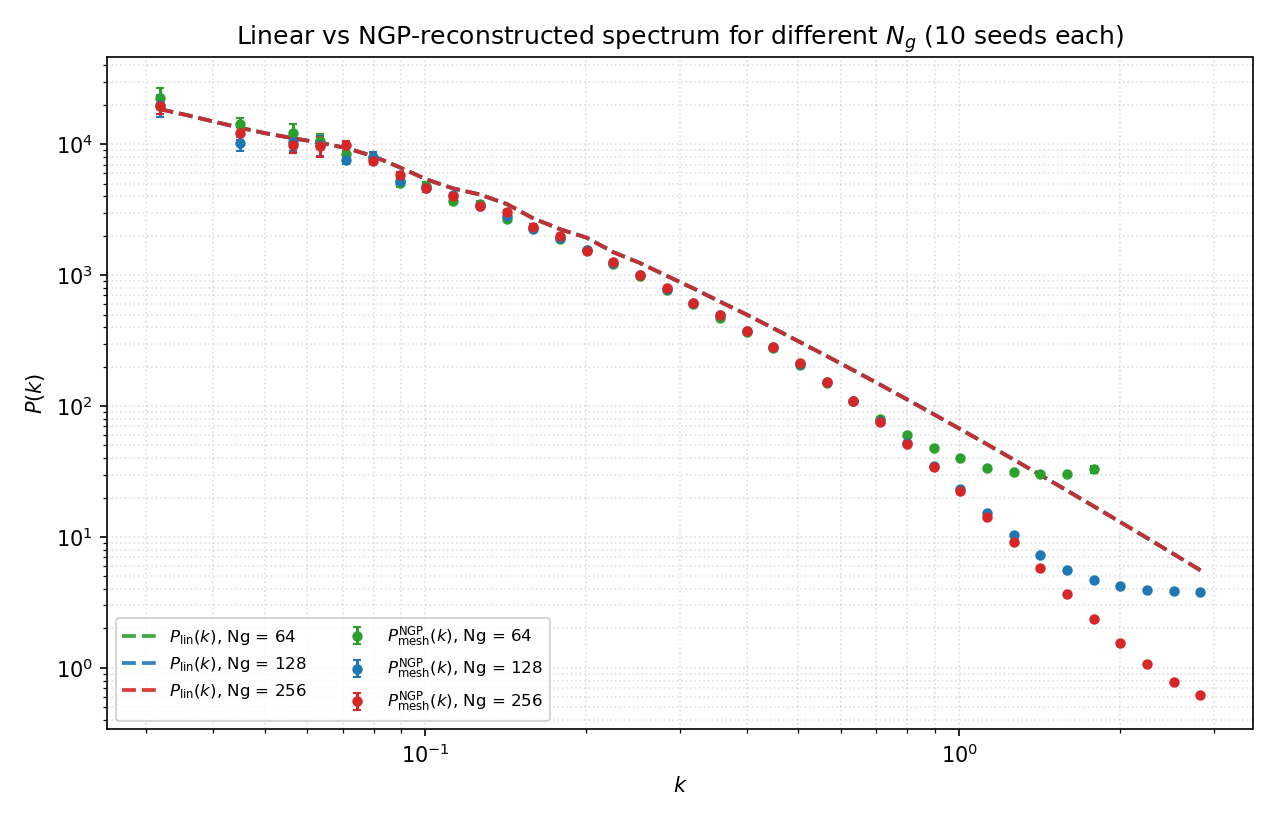
\includegraphics[width=0.82\textwidth]{Figures/ngp_multiNg_P_lin_vs_P_mesh.png}
    \caption{Comparison between the linear matter power spectrum and the averaged power spectra measured from the numerical realizations for \(N_g=64\), \(128\), and \(256\), using ten random seeds for each resolution. The mass-assignment window correction is included according to the adopted estimator.}
    \label{fig:Power_spectrum_diff_Ng}
\end{figure}

Averaging over random seeds reduces the impact of realization-dependent fluctuations and makes the resolution dependence easier to identify. The comparison with the CAMB spectrum therefore provides a quantitative test of the initial conditions and the numerical power-spectrum estimator. In particular, agreement over the range of well-resolved wavenumbers supports the consistency of the implemented first-order displacement field and the associated density-field measurement.

\subsubsection{Second-Order LPT}

The numerical validation of Second-Order Lagrangian Perturbation Theory (2LPT) is performed using the bispectrum and reduced skewness estimators introduced in Exercise 2. These statistics complement the power spectrum by characterizing the non-Gaussian features generated by nonlinear gravitational evolution.

First, we measure the bispectrum for equilateral Fourier-space triangles in the initial Gaussian field, the Zel'dovich approximation, and the 2LPT output:

\begin{figure}[H]
    \centering
    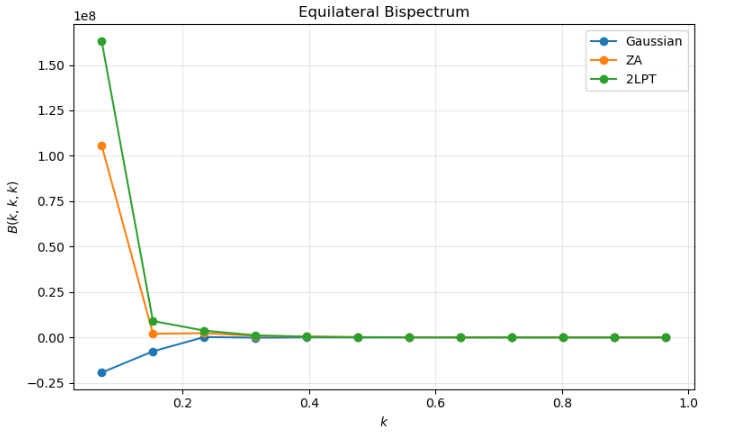
\includegraphics[width=0.82\textwidth]{Figures/equilateral_bispectrum_2LPT.png}
    \caption{Comparison of the equilateral bispectrum measured from the initial Gaussian field, the Zel'dovich approximation, and the 2LPT output.}
    \label{fig:Bispectrum}
\end{figure}

As shown in Figure (\ref{fig:Bispectrum}), the initial Gaussian field exhibits a bispectrum consistent with zero within the statistical and numerical uncertainties, as expected for an ideal Gaussian random field. In contrast, the ZA and 2LPT outputs develop nonzero bispectra, reflecting the non-Gaussian density fluctuations generated by nonlinear evolution. The bispectrum therefore provides a useful diagnostic of the nonlinear mode coupling introduced by the Lagrangian displacement field.

We further investigate the non-Gaussianity of the evolved density fields by measuring the reduced skewness as a function of the smoothing scale \(R\).

\begin{figure}[H]
    \centering
    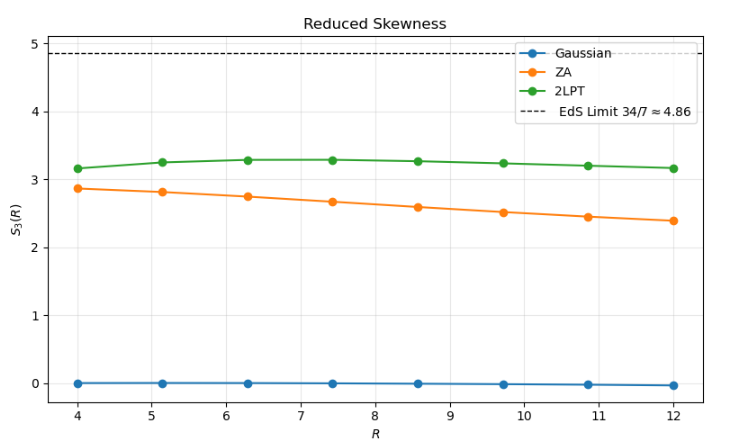
\includegraphics[width=0.82\textwidth]{Figures/Reduced_Skewness_2LPT.png}
    \caption{Comparison of the reduced skewness as a function of smoothing scale \(R\) for the initial Gaussian field, the Zel'dovich approximation, and the 2LPT output.}
    \label{fig:Reduced_Skewness}
\end{figure}

Figure (\ref{fig:Reduced_Skewness}) shows that the initial Gaussian field has reduced skewness close to zero, whereas the ZA and 2LPT density fields develop positive skewness. This behavior is consistent with the generation of non-Gaussian density statistics through gravitational evolution, which produces an increasingly asymmetric density distribution as overdense regions grow.

Taken together, the bispectrum and reduced-skewness measurements provide complementary tests of the 2LPT implementation. The bispectrum probes correlations between Fourier modes, while the skewness characterizes the asymmetry of the smoothed density distribution. Their comparison across the Gaussian, ZA, and 2LPT fields helps assess whether the numerical evolution produces the expected nonlinear statistical signatures. 